\PassOptionsToPackage{usenames,dvipsnames}{xcolor}

\documentclass[12pt,letterpaper]{book}

%Packages
\usepackage[utf8]{inputenc}
\usepackage[T1]{fontenc}
\usepackage[english]{babel}
\usepackage{amsfonts}
\usepackage{amsthm}
\usepackage{mathtools}
\usepackage{amssymb}
\usepackage{mathrsfs}
\usepackage{cancel}
\usepackage{emptypage}
\usepackage{graphicx}
\usepackage{multirow}
\usepackage[all]{xy}
\usepackage[margin=2.5cm, headheight=20pt]{geometry}
\usepackage{eso-pic}
\newcommand\BackgroundPic{%
	\put(-210,340){%
		\parbox[b][\paperheight]{\paperwidth}{%
			\vfill
			\centering
			
\includegraphics[scale=0.15,			keepaspectratio]{Escudo_unal_2016.png}%
			\vfill
}}}
\usepackage{fancyhdr}
\usepackage{enumerate}

\pagestyle{fancy}
\fancyhf{}
\fancyhead[LO]{  {\fontsize{8}{5}\textsl{\rightmark}}}
\fancyhead[RO]{  {\fontsize{8}{5}\selectfont Daniela \textsc{Martinez}} }
\fancyhead[RE]{ { \fontsize{8}{5} \textsl{\leftmark}}}
\fancyhead[LE]{ {\fontsize{8}{5} \selectfont Camilo  \textsc{Arias} }}
\fancyfoot[C]{\thepage}

\renewcommand{\headrulewidth}{1.5pt}


\usepackage{tikz}
\usetikzlibrary{cd,lindenmayersystems,arrows.meta,decorations.pathmorphing,decorations.markings,intersections}
\usepackage{imakeidx}
\makeindex[columns=2, title=Index, intoc]

%\PassOptionsToPackage{usenames,dvipsnames}{xcolor}
%\usepackage[usenames,dvipsnames]{xcolor}
\usepackage{tcolorbox}
\usepackage{fix-cm}
\usepackage{latexsym}
\usepackage{pb-diagram}
\usepackage{amsmath,amscd}
\usepackage{layout}
\usepackage{verbatim}
\usepackage{alltt}
\usepackage{bbm}
\usetikzlibrary{matrix,arrows,decorations.pathmorphing}
\usepackage{upgreek}
\usepackage{tikz-cd}
\usetikzlibrary{cd}
\usepackage{multicol}
\usepackage[hidelinks]{hyperref}



\newtheorem{theorem}{Theorem}[section]
\newtheorem{lemma}[theorem]{Lemma}
\newtheorem{proposition}[theorem]{Proposition}
\newtheorem{num}[theorem]{}
\newtheorem{corollary}[theorem]{Corollary}
\newtheorem{definition}[theorem]{Definition}
\theoremstyle{definition}
\newtheorem{example}[theorem]{Example}
\newtheorem{exercise}{Exercise}
\newtheorem{remark}[theorem]{Remark}
\newtheorem{axiom}{Axiom}
\newtheorem{note}{Note}
\newtheorem{conventions}{Conventions}
\newtheorem{free}{}
\newtheorem{notation}{Notation}
\newtheorem{obs}{Observation}
\newtheorem{observation}{Observation}
\newtheorem*{conjecture}{Conjecture}
\newtheorem*{theoremnn}{Theorem}
\newtheorem*{acknowledgements}{Acknowledgements}
\newcommand{\rmap}{\longrightarrow}
\newcommand{\Rep}{\textrm{Rep}}
\newcommand{\Der}{\textrm{Der}}
\newcommand{\RRep}{\mathcal{R}\textrm{ep}^{\infty}}
\newcommand{\URRep}{\mathcal{\hat{R}}\textrm{ep}^{\infty}}
\newcommand{\DDer}{\mathbb{D}\textrm{er}}
\newcommand{\pr}{pr}
\newcommand{\nor}{\mathrm{nor}}
\newcommand{\diff}{\mathrm{diff}}
\newcommand{\Ad}{\mathrm{Ad}}
\newcommand{\ad}{\mathrm{ad}}
\newcommand{\hPsi}{\hat{\Psi}}
\newcommand{\hR}{\hat{R}}
\newcommand{\hOmega}{\hat{\Omega}}
\newcommand{\id}{\mathrm{id}}
\newcommand{\End}{\textrm{End}}
\newcommand{\Hom}{\textrm{Hom}}
\newcommand{\RHom}{\underline{\mathrm{Hom}}}
\newcommand{\Lie}{\textrm{Lie}}
\newcommand{\smooth}{\mathcal{C}^{\infty}}
\newcommand{\Path}{\mathsf{P}}
\newcommand{\ev}{\textrm{ev}}
\newcommand{\Hoch}{\textrm{Hoch}}
\newcommand{\Chen}{\mathsf{C}}
\newcommand{\B}{\mathsf{B}}
\newcommand{\R}{\mathbb{R}}
\newcommand{\RR}{\ensuremath{\mathbb R}}
\newcommand{\MC}{\ensuremath{\mathbb C}}
\newcommand{\can}[1]{\ensuremath \cancelto{\mbox{\footnotesize 0}}{#1}}

\begin{document}
%\newgeometry{
	total={170mm,257mm},
	left=10mm,
	right=10mm,
	top=20mm,}

%\AddToShipoutPictureFG
\AddToShipoutPictureFG*{\BackgroundPic}
\thispagestyle{empty}

%\makebox[0pt][l]{%
%  \raisebox{-\totalheight}[0pt][0pt]{%
%    
\includegraphics[width=1in]{Escudo_unal_2016.png}}}%


\begin{tcolorbox}[coltext=Mahogany,colback=ForestGreen,arc=0pt,outer arc=0pt,boxrule=0.0pt,halign upper=right, height=2cm,valign=center]
 \textbf{FACULTY OF SCIENCE}
\end{tcolorbox}

\vspace{4.5cm}

\textbf{
\hspace{0.1cm} \textcolor{Mahogany}{\LARGE On Chern's conjecture} \\ 
\vspace{1cm}
\hspace{0.5cm} \textcolor{Mahogany}{ \LARGE about the Euler charateristic of affine manifolds}}

\vspace{5.5cm}

\begin{table}[ht]
\raggedleft
\begin{tabular}{lllll}
 &\textbf{\Large Daniela MARTINEZ }  & &   &
\end{tabular}
\end{table}

%\begin{flushright}
%\hspace{5cm}\large \color{black} \textbf{Daniela MARTINEZ}
%\end{flushright}



\vspace{4cm}

\begin{table}[ht]
\centering
%\caption{My caption}
\label{my-label}
\begin{tabular}{llllllr}
Promotors:   & Prof. Dr. Camilo Arias Abad       &  &  &  &  & Thesis presented in                 \\
             & National University of Colombia               &  &  &  &  & fulfillment of the requirements     \\
             &   at Medell\'in           &  &  &  &  & for the degree of Master of Science \\
             &                  &  &  &  &  & in Mathematics                                                         \\
             &                            &  &  &  &  & Academic year 2016-2017            
\end{tabular}
\end{table}



\begin{tcolorbox}[colback=Mahogany,arc=0pt,outer arc=0pt,colframe=white,boxrule=0.0pt,halign upper=right, height=0.2cm,]
 \end{tcolorbox}

\restoregeometry


\newpage{\pagestyle{empty}\cleardoublepage}

\newpage
\begin{center}
	\thispagestyle{empty} \vspace*{0cm} \textbf{\huge
		On Chern's conjecture about the Euler charateristic of affine manifolds}\\[3.0cm]
	\Large\textbf{Daniela Mart\'{i}nez Madrid}\\[3.0cm]
	\small Thesis presented in fulfillment of requirements for the degree of:\\
	\textbf{Master of Science in mathematics}\\[2.5cm]
	Promotors:\\
	Prof. Dr. Camilo Arias Abad\\[2.0cm]
	Area of Research:\\
	Differential Geometry\\
	National University of Colombia\\
	Faculty of Science, Department of Mathematics\\
	Medell\'{i}n, Colombia\\
	2017\\
\end{center}
\tableofcontents
\chapter{Introduction}
%An affine structure on a manifold is an atlas whose transition functions are affine transformations. The existence of such a structure is equivalent to the existence of a flat torsion free connection on the tangent bundle. Chern's conjecture states the following:

\begin{conjecture}[Chern $\sim$ 1955]
	The Euler characteristic of a closed affine manifold is zero.
\end{conjecture}
In case the connection $\nabla$ is the Levi-Civita connection of a riemannian metric, the Chern-Gauss-Bonnet formula:

\[ \chi(M)= \Big(\frac{1}{2\pi}\Big)^n \int_M \mathsf{Pf}(K),\]

\noindent implies that the Euler characteristic is zero. However, not all flat torsion free connections on $TM$ admit a compatible metric, and therefore, Chern-Weil theory cannot be used in general to write down the Euler class in terms of the curvature.\\

These thesis contain an exposition of the following results concerning  the Euler characteristic of affine manifolds:
\begin{itemize}
	\item In 1955, Benz\'ecri \cite{B} proved that a closed affine surface has zero Euler characteristic.
	
	\item In 1958, Milnor \cite{Milnor} proved inequalities which completely characterise those oriented rank two bundles over a surface that admit a flat connection.
	
	\item In 1975, Kostant and Sullivan \cite{KS} proved Chern's conjecture in the case where the manifold is complete.
	
	\item In 1977, Smillie \cite{Smillie} proved that the condition that the connection is torsion free matters. For each even dimension greater than $2$, Smillie constructed closed manifolds with non-zero Euler characteristic that admit a flat connection on their tangent bundle.
	
	
	
	\item In 2015, Klingler \cite{K} proved the conjecture for special affine manifolds. That is, affine manifolds that admit a parallel volume form.
	
\end{itemize}

Recently, Feng and Zhang \cite{FZ} posted a proof of the general case using the Mathai-Quillen formalism for characteristic classes. Due to lack of understanding, we will not cover their work.\\ \\
We have added appendices with preliminary material.
Appendix A contains a review of the theory of connections, curvature and the Chern-Gauss-Bonnet theorem.
Appendix B contains introductions to spectral sequences and Appendix C to sheaf theory.
\section{Affine manifolds}


\begin{definition}
	A diffeomorphism $\varphi$ between open subsets of $\R^m$ is affine if it has the form:
	\[ \varphi(x)= Ax+b,\]
	where $A \in {GL}(m,\R)$ and $b \in \R^m$.
\end{definition}

\begin{definition}
	An \index{Afffine structure} affine structure on a manifold is an atlas such that all transition functions are affine and it is maximal with this property.
	An affine manifold is a manifold together with an affine structure.
\end{definition}

It is possible to characterise affine structures in a more intrinsic manner that can be expressed without reference to an atlas, as the following lemma shows:

\begin{lemma}
	Let $M$ be a manifold. There is a natural bijective correspondence between affine structures on $M$ and flat torsion free connections on $TM$.
\end{lemma}
\begin{proof}
	Let $(U_\alpha,\varphi_\alpha)$ be an affine structure on $M$. There is a unique connection $\nabla$ on $TM$ whose Christoffel symbols vanish in affine coordinates. Conversely, given a flat torsion free connection $\nabla$ on $TM$, the set of coordinates for which the Christoffel symbols of $\nabla$ vanish gives an affine structure on $M$.
\end{proof}

\begin{example}
	The torus $\mathbb{T}^m:= \R^m/\mathbb{Z}^m$ has a natural affine structure for which the projection map $\pi: \R^m \rightarrow \mathbb{T}^m$ is an affine local difeomorphism.
\end{example}


\begin{example}[Hopf manifolds]
	Let us fix a real number $\lambda>1$ and consider the action of the group $\mathbb{Z}$ on $\R^m-\{0\}$ given by:
	\[ n \star x:= \lambda^n x.\]
	Since the action is free and proper, the quotient is a smooth manifold called the Hopf manifold $\mathsf{Hopf}^m_\lambda$. Since the group $\mathbb{Z}$ acts by affine transformations the quotient space is an affine manifold. Topologically, these manifolds are the union of two circles for $m=1$ and diffeomorphic to $S^{m-1}\times S^1$ for $m>1$.
\end{example}


\begin{definition}
	An affine structure on a Lie group $G$ is called left invariant if for all $g \in G$:
	\[ (L_g)^*(\nabla)=\nabla,\]
	where $L_g$ denotes the diffeomorphism given by left multiplication by $g$.
\end{definition}

\begin{definition}
	Let $V$ be a real vector space. A bilinear map:
	\[\beta: V \otimes V \rightarrow V;\,\, v \otimes w \mapsto v\cdot w\]
	is called left symmetric if:
	\[ v\cdot (w \cdot z)-(v\cdot w) \cdot z= w\cdot (v \cdot z)-(w\cdot v)\cdot z.\]
\end{definition}


\begin{definition}
	An affine structure on a finite dimensional real Lie algebra $\mathfrak{g}$ is a left symmetric bilinear form on $\mathfrak{g}$ such that for all $v,w \in \mathfrak{g}$:
	\[ [v,w]=v\cdot w- w \cdot v.\]
\end{definition}

\begin{lemma}
	Let $G$ be a Lie group with Lie algebra $\mathfrak{g}$. There is a natural bijective correspondence between
	left invariant affine structures on $G$ and affine structures on $\mathfrak{g}$.
\end{lemma}

\begin{proof}
	For any $v \in \mathfrak{g}=T_eG$ denote by $\hat{v}$ the corresponding left invariant vector field. Given a left invariant affine structure on $G$ we define a bilinear form on $\mathfrak{g}$ by:
	\[ v\cdot w:= \nabla_{\hat v}\hat{w}(e).\]
	Since $\nabla$ is torsion free we know that:
	\[ v \cdot w - w \cdot v =  \nabla_{\hat v}\hat{w}(e)-  \nabla_{\hat w}\hat{v}(e) =[v,w].\]
	Using the fact that $\nabla$ is flat and left invariant, we compute:
	\begin{eqnarray*}
		v\cdot (w \cdot z)-(v\cdot w) \cdot z-w\cdot (v \cdot z)+(w\cdot v)\cdot z&=& \nabla_{\hat{v}} (\nabla_{\hat{w}}(\hat{z}))\\
		&\quad&-\nabla_{\nabla_{\hat{v}}(\hat{w})}(\hat{z}) - \nabla_{\hat{w}} (\nabla_{\hat{v}}(\hat{z}))+\nabla_{\nabla_{\hat{w}}(\hat{v})}(\hat{z})\\
		&=&\nabla_{[\hat{v},\hat{w}]}(\hat{z})-\nabla_{[\hat{v},\hat{w}]}(\hat{z})\\
		&=&0.
	\end{eqnarray*}
	So we conclude that the bilinear form is left symmetric. Conversely, given an affine structure on $\frak{g}$ there is a unique left invariant connection $\nabla$ such that:
	\[ \nabla_{\hat{v}}\hat{w}(e)=v\cdot w.\]
	The computations above show that this connection is flat and torsion free.
\end{proof}

\begin{example}
	The Lie algebra $\mathfrak{gl}(n,\R)$ admits a natural affine structure given by:
	\[ A \cdot B:= AB.\]
	We conclude that the Lie group $GL(n, \R)$ admits a left invariant affine structure.
\end{example}


The question of which Lie groups admit left invariant affine structures is an interesting problem. In \cite{Milnor2}, Milnor asked whether solvable Lie algebras admit affine structures. In \cite{Bu}, Burde showed that the answer to this question is negative.

\section{Complete manifolds and the developing map}

In this section we introduce the developing map of a simply connected affine manifold and use it to characterise complete affine manifolds.

\begin{theorem}
	Let $M$ be an affine manfiold of dimension $m$ and $G$ be the group $\mathsf{Aff}(\mathbb{R}^m)$ seen as a discrete group. There is a natural principal $G$-bundle \linebreak{ $\pi:\tau(M) \rightarrow M$} such that sections  of $\pi$ are in natural bijective correspondence with affine immersions from $M$ to $\R^m$. \end{theorem}
\begin{proof} For each $p\in M$ we define:
	\[C_{p}= \left\{  \varphi: U\to V\subseteq \R^m:  \varphi \text{ is an affine diffeomorphism and }p\in U \right\}.\]
	
	There is an equivalence relation $\sim$ on $C_p$ given by declaring that $\varphi \sim \varphi'$ if an only if there exists an open subset $W \subseteq U \cap U'$ such that $p \in W$ and $\varphi\vert_W=\varphi' \lvert_W$. Let us denote by $L_p$ the set of equivalence classes of elements in $C_p$ and set:
	\[\tau(M):=\coprod_{p} L_{p}.\]
	There is a natural map:
	\[
	\pi:\tau(M) \rightarrow M . \]
	The Lie group $G$ acts on each set $L_p$ by composition:
	\[g \ast \varphi := g \circ \varphi,\]
	and this action is free and transitive. Moreover, an affine chart $\varphi: U \rightarrow V\subseteq \R^m$ induces a natural identification:
	\[ \hat{\varphi}: \mathsf{Aff}(\R^m)\times U \rightarrow \pi^{-1}(U); \,\, (g,p)\mapsto [ g \circ \varphi]_p, \]
	where $[g \circ \varphi]_p$ denotes the class of $g \circ \varphi$ in $L_p$. There is a unique topology on $\tau(M)$ such that $\hat{\varphi}$ is a homeomorphism for all affine diffeomorphisms $\varphi$. The map $\pi: \tau(M) \rightarrow M$ is a principal $G$ bundle with respect to this topology. Let $\sigma$ be a section of $\pi$. Then we define $\tilde{\sigma}:M \rightarrow \R^m$ by:
	\[ \tilde{\sigma}(p):= \sigma(p) (p).\]
	By construction, the map $\tilde{\sigma}$ is an affine immersion. Conversely, an affine immersion \linebreak{ $f: M \rightarrow \R^m$} defines a section $\sigma_f$ given by:
	\[ \sigma_f(p):= [f]_p.\]
\end{proof}


\begin{corollary}\label{extend}
	Let $M$ be a simply connected affine manifold. Any affine chart \linebreak{ $\varphi: U \rightarrow V \subseteq \R^m$} extends uniquely to an affine immersion from $M$ to $\R^m$. \end{corollary}

\begin{proof}
	Since $M$ is simply connected, the covering space $\pi: \tau(M) \rightarrow M$ is trivial and therefore any local section extends uniquely to a global one.
\end{proof}

\begin{definition} \index{Developing map}
	A developing map for an affine simply connected manifold is an affine immersion into $\R^m$.
\end{definition}

\begin{corollary}
	If $M$ is an affine connected manifold with finite fundamental group then $M$ is not compact.
\end{corollary}

\begin{proof}
	If $M$ is compact then so is its universal cover $\tilde{M}$ which is simply connected and therefore admits an immersion to $\R^m$. This is impossible.
\end{proof}

\begin{definition} \index{Complete manifold}
	An affine manifold $M$ with affine connection $\nabla$ is called complete if all geodesics can be extended to arbitrary time.
\end{definition}

\begin{lemma}\label{unique}
	Let $M$ and $N$ be connected affine manifolds of the same dimension and $f,g:M \rightarrow N$ affine immersions. If $f$ and $g$ coincide on a nonempty open subset of $M$ then they are equal.
\end{lemma}
\begin{proof}
	First we observe that the lemma is true if $M$ and $N$ are open subsets of $\R^m$.
	For the general case, let $X\subset M$ be the subset of $M$ that consists of points $p\in M$ such that $f$ and $g$ coincide in an open neighborhood of $p$. Clearly, $X$ is open. It suffices to show that $X$ is closed.
	Fix $p \in X$ and $q \in M$ arbitrary. Since $M$ is connected, there is a path $\gamma: I \rightarrow M$ such that
	$\gamma(0)=p$ and $\gamma(1)=q$. Set \[Y:= \gamma^{-1}(M-X).\] We would like to show that $Y=\emptyset$. Suppose that $Y$ is nonempty and set $y:=\inf(Y)$ and $z=\gamma(y)$. Choose affine coordinates $\varphi: U \rightarrow V$ around $z$ and $ \psi: W \rightarrow Z $ around $f(z)$ such that $f(U) \subseteq W$ and $g(U) \subseteq W$. Since $p$ is in $X$ there exists $l<y$ such that $\gamma(l) \in U\cap X$. Then $f\vert_U$ and $g\vert_U$ coincide in an open neighborhood. Since both $U$ and $ W$ are isomorphic to open subsets of $\R^m$ we conclude that $f\vert_U=g\vert_U$. This is a contradiction.
\end{proof}


\begin{lemma}\label{local}
	Let $M$ be a simply connected complete affine manifold of dimension $m$. Then any affine coordinate $\varphi: U \rightarrow V\subseteq \R^m$ can be extended uniquely to a diffeomorphism from $M$ to $\R^m$.
\end{lemma}
\begin{proof}
	Fix a point $p \in M$ and affine coordinates $\varphi: U \rightarrow V$. By Corollary \ref{extend},
	$\varphi$ can be extended uniquely to an affine immersion $\tilde{\varphi}: M \rightarrow \R^m$. We will prove that $\tilde{\varphi}$ is a diffeomorphism. Since $M$ is complete, the exponential map is defined on the whole tangent space $T_pM$:
	\[ \mathsf{Exp}: T_pM \rightarrow M.\]
	On the other hand, the derivative of $\varphi^{-1}$ at $x=\varphi(p)$ is an isomorphism from $\R^m$ to $T_pM$. We claim that
	the map: \[\psi(y):=\mathsf{Exp} \circ D(\varphi^{-1})(y-x)\]
	is the inverse of $\tilde{\varphi}$. By Lemma \ref{local}, it suffices to show that the functions are inverses to each other in a small open neighborhood. For $q \in U$ we compute:
	\[ \psi (\tilde{\varphi}(q))= \mathsf{Exp} \circ D(\varphi^{-1})(\varphi(q)-x)=q.\]
	Conversely, for $y \in V$ we have:
	\[ \tilde{\varphi}\circ \psi(y)= \varphi \circ \mathsf{Exp} \circ  D(\varphi^{-1})(y-x)= \mathsf{Exp}(y-x)=y. \]
\end{proof}


\begin{proposition}\label{develop} \index{Complete manifold}
	Let $M$ be an affine manifold. The following statements are equivalent:
	\begin{enumerate}
		\item  $M$ is complete.
		\item There is an affine diffeomorphism $M \cong \R^m /\Gamma$, where $\Gamma$ is a discrete subgroup of $\mathsf{Aff}(\R^m)$ and the projection $\pi: \R^m \rightarrow M$ is the universal cover of $M$.
	\end{enumerate}
\end{proposition}

\begin{proof}
	Let us assume that $M$ is complete. Then $\tilde{M}$ is also complete and simply connected. By Proposition \ref{develop} there is an affine difeomorphism $\varphi: \tilde{M} \rightarrow \R^m$. Let us fix a point $p \in M$. Then there is an action of $\pi_1(M,p)$ on $\tilde{M}$ and therefeore on $\R^m$. Since this action is by affine transformations, it defines a homomorphism $\rho: \pi_1(M,p) \rightarrow \mathsf{Aff}(\R^m)$. If we set $\Gamma:= \mathsf{Im}(\rho)$ we get by construction that $ M \cong \R^m/\Gamma$. Conversely, any manifold of the form $\R^m/\Gamma$ is complete.
	
	
\end{proof}
\chapter{Milnor's inequalities and the conjecture in dimension $d=2$}
%Throughout this section we will set $G=GL^{+}(2,\R)$, $S=SO(2)=U(1)$ and $\Sigma$ will be a closed oriented surface of positive genus $g$. 
Oriented rank two vector bundles over $\Sigma$ are classified by their Euler class. Milnor considered the question
of which of those bundles admit a flat connection. The answer is given by his famous inequalities, which are the following. 

\begin{definition}
	Let $\pi: E \rightarrow \Sigma$ be a rank two oriented vector bundle. The degree of $E$ is the number:
	\[ D(E)= \int_\Sigma e(E).\]
	Here $e(E)$ denotes the Euler class of $E$.
\end{definition}

\begin{theoremnn}
	A rank two oriented vector bundle $\pi:E \rightarrow \Sigma$ admits a flat connection if and only if:
	\[ |D(E)|<g.\]
\end{theoremnn}



Milnor's inequalities give in particular a positive answer to Chern's conjecture in dimension $d=2$, a result that had been previously obtained by Benzecri \cite{B}.

The classification of rank two oriented bundles is of course the same as the classification of $GL^{+}(2,\R)$ principal bundles. 

\begin{lemma}
	The inclusion $\iota: S \hookrightarrow G$ is a homotopy equivalence and therefore the classifying spaces $BS$ and $BG$ are homotopy equivalent.
\end{lemma}
\begin{proof}
	By the spectral theorem every nonsingular matrix $\gamma$ can be written uniquely in the form $\gamma=OS$, where $O$ is orthogonal matrix and $S$ is symmetric positive definite matrix. Then the following function define a retraction:
	$$
	\begin{array}{rcc}
	\theta :G & \longrightarrow & S\\
	\gamma & \longmapsto & O.
	\end{array}
	$$
\end{proof}


\begin{lemma}
	Let $\mathsf{Bun}(\Sigma)$ be the set of isomorphism classes of rank two oriented vector bundles over $\Sigma$. The degree:
	\[D: \mathsf{Bun}(\Sigma) \rightarrow \mathbb{Z}; \, E \mapsto D(E)\]
	is bijection.
\end{lemma}
\begin{proof}
	The set $\mathsf{Bun}(\Sigma)$ is in bijective correspondence with the set of isomorphism classes of principal $G$ bundles over $\Sigma$. These are 
	classified by the set $[\Sigma, BG]$ of homotopy classes of maps to $BG$. Moreover:
	\[[\Sigma,BG]\cong[\Sigma,BS]\cong[\Sigma,\mathbb{CP}^{\infty}]=[\Sigma,K(\mathbb{Z},2)]\cong H^2(\Sigma,\mathbb{Z}) \cong \mathbb{Z}.\]
	By definition of the Euler class, this bijection is given by the degree.
\end{proof}

\begin{exercise}
	Fix a point $p \in \Sigma$ and a homomorphism $\rho: \pi_1(\Sigma, p) \rightarrow G$. The group \linebreak{$\pi=\pi_1(\Sigma,p)$} acts on the right on the universal cover $\tilde{\Sigma}$ and on the left on $\R^2$ via the representation $\rho$. Let $\tilde{\Sigma}\times_\rho V$ be the quotient of $\tilde{\Sigma} \times V$ via the equivalence relation:
	\[ (m g,v)\sim (m,\rho(g)v).\]
	Show that $\tilde{\Sigma}\times_\rho V$ has a natural structure of a flat oriented vector bundle over $\Sigma$. We will denote this vector bundle $E^\rho$ and call it the bundle associated to $\rho$.
\end{exercise}


\begin{lemma}
	A vector bundle over $\Sigma$ admits a flat connection if an only if it is isomorphic to one of the form $E^\rho$.
\end{lemma}

\begin{proof}
	By the previous exercise, $E^\rho$ admits a flat connection. Assume that $E$ admits a flat connection $\nabla$ and fix a point $p \in \Sigma$ and an isomorphism $E_p\cong \R^2$. The holonomy of $\nabla$ gives a representation $\rho: \pi_1(\Sigma, p) \rightarrow G$ and an isomorphism \linebreak{$E \cong E^\rho$.}
\end{proof}



An oriented closed surface $\Sigma$ of genus $g$ admits a CW structure with one zero-dimensional cell, $2g$  one-dimensional cells and one two-dimensional cell. For example, the surface of genus $2$ can be obtained by the following identification:
\begin{center}
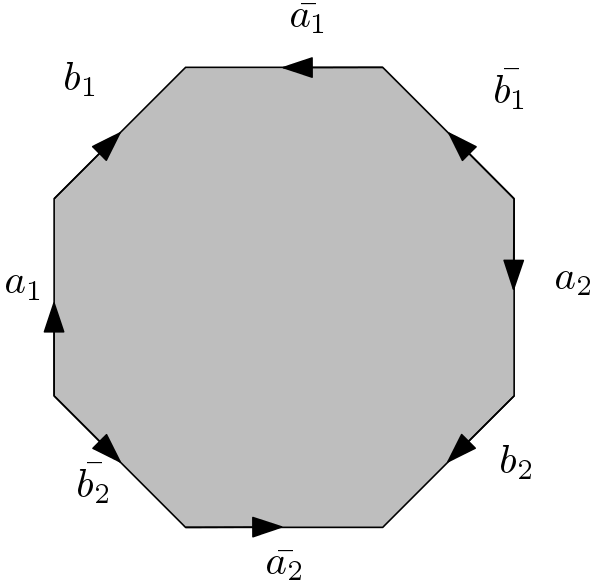
\includegraphics[scale=0.2]{imatesis.png}
\end{center}

In general, this decomposition gives the following presentation of the fundamental group of $\Sigma$:
\[\pi_1(\Sigma)=\bigg{\langle} a_1,\dots, a_g, b_1, \dots, b_g \quad | \quad \prod_{i=1}^g [a_i,b_i]=1 \bigg{\rangle}, \]
here $[a,b]$ denotes the commutator $aba^{-1}b^{-1}$. Thus, a representation $\rho$ of $\pi_1(\Sigma)$ on $G$ is the same as a choice of matrices
$A_1,\dots,A_g,B_1, \dots B_g \in G$ such that \[\prod_{i=1}^g [A_i,B_i]=\id.\]
We have seen that such a representation gives rise to a vector bundle $E^\rho$ and the natural question arises of computing the degree of $E^\rho$ in terms of
the matrices $A_i, B_i$.


Let $\tilde{G}$ be the universal cover of $G$ and consider the short exact sequence  
\[0 \rightarrow \pi_1(G) \xrightarrow{\iota} \tilde{G} \xrightarrow{p} G \rightarrow 0.\]

Consider also the map $\phi: \R \rightarrow S$ given by:

$$\begin{array}{rcc}
\alpha & \longmapsto & \left[ {\begin{array}{cc}
	\cos \alpha & \sin \alpha\\
	-\sin \alpha & \cos \alpha \\
	\end{array} }  \right] .
\end{array}$$

The map $\phi$ is the universal covering map of $S$ and therefore the retraction map $\theta: G \rightarrow S$ can be lifts naturally to a map:
\[ \hat{\theta}: \tilde{G} \rightarrow \R.\]

Thus we obtain the following commutative diagram:
\begin{center}
	\begin{tikzcd}
		& 0 \arrow[d] & 0 \arrow[d] &  \\
		& \pi_1(G) \arrow[r] \arrow[d,"\iota"] & \mathbb{Z} \arrow[d, "2 \pi"] & \\
		& \tilde{G} \arrow[r, "\tilde{\theta}"] \arrow[d,"p"] & \mathbb{R}  \arrow[d,"\phi"] &\\
		\pi_1(\Sigma) \arrow [r, "\rho"]	&G \arrow[r,"\theta"]  & S &
	\end{tikzcd}	
\end{center}


\begin{lemma}
	Given a homomorphism $\rho: \pi_1(\Sigma) \rightarrow G$ determined by matrices $A_1, \dots, A_g, B_1,\dots, B_g$ we define the number $\delta(\rho)$ by:
	\[ \delta(\rho):= \frac{1}{2\pi}\tilde{\theta}(\prod_{i=1}^g [\alpha_i,\beta_i])\in \mathbb{Z}.\]
	Here $\alpha_i, \beta_i$ are elements in $\tilde{G}$ such that $p(\alpha_i)=A_i$ and $p(\beta_i)=B_i$. This number depends only on $\rho$.
\end{lemma}
\begin{proof}
	Let us first proof that for any choice of the $\alpha_i$ and $\beta_i$ the number $\delta(\rho)$ is an integer. By construction, $\prod_{i=1}^g [\alpha_i,\beta_i] \in \mathsf{ker}(p)$. This implies that $\hat{\theta}(\prod_{i=1}^g [\alpha_i,\beta_i])$ is a multiple of $2\pi$ and the result follows. Let us now show that the number is well defined. Suppose that $\alpha_i'$ and $\beta_i'$ is a different choice. Then, for each $i$ we know that:
	\[ \alpha_i'=\alpha_i x_i\;\, \beta_i'= \beta_i y_i ,\]
	where the $x_i$ and the $y_i$ are in the kernel of $p$ which is contained in the center of $\tilde{G}$. This implies that:
	\[ [\alpha_i, \beta_i]=[\alpha_i',\beta_i'],\]
	and the result follows.
\end{proof}
\begin{lemma}
	Given a representation $\rho: \pi_1(\Sigma) \rightarrow G$ we have:
	\[ \delta(\rho)=D(E^\rho).\]
\end{lemma}

\begin{proof}
	This will be added later.
\end{proof}

\begin{exercise}\label{trace}
	Show that if
	\[A= \left( {\begin{array}{cc}
		a & b\\
		c & d \\
		\end{array} } \right) \in G,\] then 
	\[\theta(A)=\frac{1}{\sqrt{x^{2}+y^{2}} } \left( {\begin{array}{cc}
		x & y\\
		-y &  x \\
		\end{array} } \right). \]
	Here $x=a+d$ and $y=b-c$.
	Moreover, show that:			
	\begin{enumerate}
		\item If $A \in G$ has positive trace, then $\theta(A)$ has positive trace.
		\item If $A$ and $B$ are symmetric and positive definite matrices, then $AB$ has positive trace.
		\item If $A,B \in G$ are symmetric and positive definite matrices, then $\theta(A B)$ has positive trace.
		\item $\theta(A^{-1})=\theta(A)^{-1}$.
	\end{enumerate}
\end{exercise}




\begin{lemma}\label{angle}
	The function $\tilde{\theta}: \tilde{G} \to \mathbb{R} $ satisfies the property:
	\[|\tilde{\theta}(\alpha \beta)-\tilde{\theta}(\alpha)-\tilde{\theta}(\beta)|<\pi/2.\]
\end{lemma}
\begin{proof}
	Given $A,B\in G$, then there exists symmetric positive definite matrices $R,T$ such that:  	
	\[AB=\theta(A)R \theta(B)T.\]
	If we set $X=\theta(B)^{-1}R\theta(B)$ then:
	\[AB=\theta(A)\theta(B)XT.\]
	This implies that: \[\theta(AB)=\theta(A)\theta(B)\theta(XT).\] 
	Therefore:
	\[\theta(B)^{-1}\theta(A)^{-1}\theta(AB)=\theta(XT) .\]
	Since $X,T$ are positive definite, the previous Exercise \ref{trace} implies that $\theta(B)^{-1}\theta(A)^{-1}\theta(AB)$ has positive trace.
	Fix $\alpha, \beta \in \tilde{G}$ such that $p(\alpha)=A$ and $p(\beta)=B$ and 
	set $\Delta=\tilde{\theta}(\alpha \beta)-\tilde{\theta}(\alpha)-\tilde{\theta}(\beta)$. Then:
	\[ \phi(\Delta)=\left[ {\begin{array}{cc}
		\cos \Delta & \sin \Delta \\
		-\sin \Delta & \cos \Delta \\
		\end{array} } \right]=\theta(B)^{-1}\theta(A)^{-1}\theta(AB)\]
	has positive trace. So $cos \Delta >0$. Since $\Delta$ is a continuous function of $\alpha$ and $\beta$ which vanishes when $\alpha=\beta=1$ we conclude that
	$|\Delta|<\frac{\pi}{2}$.
	
	
\end{proof}


\begin{lemma}\label{bound}
	Given a representation $\rho: \pi_1(\Sigma) \rightarrow G$ we have:
	\[ |\delta(\rho)|<g.\]
\end{lemma}

\begin{proof}
	Applying Lemma \ref{angle} $4g-1$ times one obtains:
	\[|\tilde{\theta}([\alpha_1,\beta_1]\dots [\alpha_g,\beta_g] )-\tilde{\theta}(\alpha_{1})-\tilde{\theta}(\beta_{1})-\tilde{\theta}(\alpha_{1}^{-1})-\tilde{\theta}(\beta^{-1}_1) \dots-\tilde{\theta}(\alpha_{g})-\tilde{\theta}(\beta_{g})-\tilde{\theta}(\alpha_{g}^{-1})-\tilde{\theta}(\beta^{-1}_g)  | \]
 	 \[	<(4g-1)\frac{\pi}{2}\] 
	By Exercise \ref{trace} we know that 
	\[\tilde{\theta}(\alpha)+\tilde{\theta}(\alpha^{-1})=0,\]
	so that the inequality above becomes:
	\[|\tilde{\theta}([\alpha_1,\beta_1]\dots [\alpha_g,\beta_g])  |<(4g-1)\frac{\pi}{2}.\]
	
	Dividing by $2\pi$ one obtains:
	\[ |\delta(\rho)|<g-\frac{1}{4}<g.\]
	
\end{proof}

The lemma gives one direction of Milnor's inequalities. We will now show that the converse is also true.

\begin{exercise}\label{center}
	Let $G$ be a connected Lie group with universal cover $\tilde{G}$. Show that if $g \in \tilde{G}$ is such that $p(g) \in Z(G)$ then $g \in Z(\tilde{G})$.
\end{exercise}





Let us set $A_{0}:= \left( \begin{array}{cl} 
2 & 0 \\
0 & 1/2
\end{array} \right)  $                    and   $\alpha_{0} \in p^{-1}(A_{0})$ so that $\tilde{\theta}(\alpha_{0})=0$.
We will denote by $K$ and $\tilde{K}$ the conjugacy classes of $A_{0}$ and $\alpha_{0}$ respectively. \\

Since $\R$ is simply connected, the group homomorphism $\phi: \R \rightarrow G$ lifts to a homomorphism $\R \rightarrow \tilde{G}$ and therefore
$\R$ acts on $\tilde{G}$ and also on conjugacy classes of $\tilde{G}$.





\begin{lemma}\label{product}
	Any element of $\pi \tilde{K}$ can be written as a product of two elements in $\tilde{K}$.
\end{lemma}
\begin{proof}
	Consider the matrices:
	
	\[A_{1}=\left(  \begin{array}{cl}
	-5/2 & 9/2\\
	-3 & 5
	\end{array}\right)\] and 
	\[A_{2}=A_{0} A_{1} =
	\left( \begin{array}{cl}
	-5 & 9\\
	-3/2 & 5/2
	
	\end{array}\right).\]
	
	Since the trace and determinant characterise the sets ${K}$ and $ \pi K$,
	then $A_{0}, A_{1} \in K$ and  $A_{2} \in \pi K$.
	Let  $\alpha_{0},\alpha_{1} \in \tilde{K} $ be such that $p(\alpha_i)=A_i$ and $\tilde{\theta}(\alpha_{i})=0$. Then $\alpha_{0} \alpha_{1} \in  n\pi \tilde{K}$ for some odd integer $n$. Let us show that $n=\pm1$.
	Given  $\alpha \in \tilde{K}$ we know that $p(\alpha)$ has positive trace and therefore $\cos(\tilde{\theta}(\alpha))>0$.
	Therefore, if $\beta \in n\pi \tilde{K}$ with $|n|>1$ then:
	
	\[|\tilde{\theta}(\beta)|>\frac{5\pi}{2}.\]
	Applying Lemma \ref{angle} we obtain:
	
	\[ |\tilde{\theta}(\alpha_{0} \alpha_{1})|< |\tilde{\theta}(\alpha_{0})|+|\tilde{\theta}(\alpha_{1})| + \frac{\pi}{2} < \frac{3}{2} \pi \]
	
	We conclude that $n=\pm1$.
	\begin{itemize}
		\item If $n=1$ we set:\[\gamma(\alpha_{0} \alpha_{1})\gamma^{-1}=(\gamma \alpha_{0} \gamma^{-1})(\gamma \alpha_{1} \gamma^{-1}) \in \tilde{K}\tilde{K}.\]
		\item If $n=-1$ then $\gamma(\alpha_{0} \alpha_{1})\gamma^{-1} \in -\pi \tilde{K}$ and $\gamma(\alpha_{0} \alpha_{1})^{-1} \gamma^{-1} \in \pi \tilde{K}$. We then write:
		\[\gamma(\alpha_{0} \alpha_{1})^{-1}\gamma^{-1}=(\gamma \alpha_{1}^{-1} \gamma^{-1})(\gamma \alpha_{0}^{-1}\gamma^{-1}) \in \tilde{K} \tilde{K}.\]
	\end{itemize}
\end{proof}

\begin{lemma}\label{lema_3}
	For every $\alpha \in \pi \tilde{K}$ there exists $\beta_1 \beta_{2} \in \tilde{G}$ so that $\alpha=\beta_{1}\beta_{2}\beta_{1}^{-1}\beta_{2}^{-1}$.
\end{lemma}
\begin{proof}
	By the previous lemma there exists $\beta_{1},\beta_{3} \in \tilde{K}$ so that $\alpha=\beta_{1}\beta_{3}$. Since $\alpha_{1} ^{-1} \in \tilde{K}$ there exists $\beta_{2} \in \tilde{G}$ so that $\beta_{2} \alpha_{1}^{-1} \beta_{2}^{-1}=\beta_{3}$.\\
	Then $$\alpha=\beta_{1} \beta_{3}=\beta_{1} \beta_{2} \beta_{1}^{-1}\beta_{2}^{-1}$$
\end{proof}
\begin{lemma}\label{list}
	For every $n \geq1 $ there exists $\gamma_1,\dots, \gamma_{n+1} \in \tilde{K}$ so that $\gamma_1 \dots \gamma_{n+1}=n \pi\alpha_{0}.$
\end{lemma}
\begin{proof}
	We will argue by induction. The case $n=1$ is Lemma \ref{product}. Now assume that the lemma holds for $n$ so that we can write:
	\[\gamma_1 \dots \gamma_{n+1}=n \pi\alpha_{0}.\] Then:
	
	\[ (n+1)\pi \alpha_0= \pi (n \pi) \alpha_0=\pi (\gamma_1 \dots \gamma_{n+1})=(\pi \gamma_1) \dots \gamma_{n+1}=\gamma \gamma' \gamma_2 \dots \gamma_{n+1}.\]
	Here $\gamma, \gamma' \in \tilde{K}$ and we have applied the Lemma product to $\pi \gamma_1$.
	
\end{proof}





\begin{theorem}\label{Milnor}
	A rank two oriented vector bundle $\pi:E \rightarrow \Sigma$ admits a flat connection if and only if:
	\[ |D(E)|<g.\]
\end{theorem}

\begin{proof}
	One direction is guaranteed by Lemma \ref{bound}. We want to prove that a bundle $E$ with $|D(E)|<g$ admits a flat connection. It suffices to show that
	there is some representation $\rho: \pi_1(\Sigma) \rightarrow G$ such that $\delta(\rho)=D(E)$. Since the existence of a flat connection does not depend on the orientation we may assume that $D(E)>0$. Since some of the matrices in the representation can be set to $\id$ it suffices to show the case where $D(E)=g-1$ and $g>1$.
	By Lemma \ref{list} there exist $\gamma_{1},...,\gamma_{g-1} \in \tilde{K}$ so that:
	\[\gamma_1 \dots \gamma_{g-1}=(g-2) \pi\alpha_{0}.\]
	
	If we set $\gamma_g=\alpha_{0}^{-1}$ then:
	\[\gamma_1 \dots \gamma_{g-1}\gamma_g=(g-2) \pi.\]
	
	Now by Lemma \ref{lema_3}, for every $1 \leqslant i \leqslant g$ there exists $\alpha_i,\beta_i \in \tilde{G}$ so that 
	\[[\alpha_i,\beta_i]= \pi \gamma_i.\]
	Then 
	\[\prod_{i=1}^g[\alpha_i,\beta_i]=2\pi (g-1).\]
	
	This implies that by setting $A_i=p(\alpha_i)$ and $B_i=p(\beta_i)$ one obtains a representation $\rho$ such that:
	\[\delta(\rho)=\frac{1}{2\pi}\prod_{i=1}^g[\alpha_i,\beta_i]= g-1.\]
\end{proof}


\begin{corollary}
	The torus is the only closed oriented surface that admits an affine structure. In particular, Chern's conjecture holds in dimension $d=2$.
\end{corollary}
\begin{proof}
	Since $S^2$ is simply connected, a flat connection on $TM$ would give a trivialization of $TM$, which does not exist because the Euler characteristic of the sphere is $2$.
	Let us now assume that $g>1$. Then $D(TM)=\chi(\Sigma)=2-2g$. Then:
	\[|D(TM)|= 2|(1-g)|=2g-2 \geq g.\]
\end{proof}

\chapter{The counterexamples of Smillie}
%\input{Cap3/cap3}
\chapter{The case of complete manifolds, after Sullivan and Kostant}
%\input{Cap4/cap4}
\chapter{Appendix}
%\section{Connection on a vector bundle}


Given a smooth function $f=(f^{1},\dots,f^{m}):M\rightarrow\mathbb{R}^{m}$ and
a vector field $X\in\mathfrak{X}(M)$ it makes sense to consider the derivative
of $f$ in the direction of $X$:
\[
X(f)=(X(f^{1}),\dots,X(f^{m}))=Df (X).
\]


On the other hand, if $\alpha\in\Gamma(E)$ is a section of a vector bundle
$E$, there is no natural way to differentiate $\alpha$ in the direction of a
vector field. A connection on a vector bundle $E$ is a rule that prescribes
how to differentiate sections of $E$ in the direction of vector fields.

\begin{definition}
	Let $\pi:E\rightarrow M$ be a vector bundle. A connection $\nabla$ on $E$ is a
	linear map:
	\[
	\nabla:\mathfrak{X}(M)\otimes\Gamma(E)\rightarrow\Gamma(E);\quad
	(X,\alpha)\mapsto\nabla_{X}\alpha
	\]
	such that for any smooth function $f\in C^{\infty}(M)$, $X\in\mathfrak{X}(M)$
	and $\alpha\in\Gamma(E)$ the following two conditions are satisfied:
	\begin{enumerate}
		\item \[\nabla_{fX}\alpha=f\nabla_{X}\alpha,\]
		\item \[\nabla_{X}\left(  f\alpha\right)  =\left(  X(f)\right)  \alpha
		+f\nabla_{X}\alpha.\]
	\end{enumerate}
\end{definition}

\begin{exercise}
	Show that in the case where $E=M \times\mathbb{R}^{m}$ is the trivial bundle,
	the directional derivative described above is a connection on $E$.
\end{exercise}

\begin{definition}
	If $E$ is a vector bundle with connection, we will say that a section
	$\alpha\in\Gamma(E)$ is covariantly constant if $\nabla_{X}(\alpha)=0$ for any
	vector field $X\in\mathfrak{X}(M)$.
\end{definition}

Let us now consider the case $E=TM$ and describe how a connection is expressed
in local coordinates $\varphi=(x^{1},\dots,x^{m})$. The Christoffel symbols
$\Gamma_{ij}^{k}:M\rightarrow\mathbb{R}$ are smooth functions determined by
the condition \[\nabla_{\partial_{i}}{\partial_{j}}=\sum_{k}%
\Gamma_{ij}^{k}\partial_{k}.\]
The connection $\nabla$ is
determined by the Christoffel symbols. Given vector fields
$X=\sum_{i}a^{i}\partial_{i},$ $Y=\sum_{j}b^{j}\partial_{j}$ one computes:
\begin{align*}
\nabla_{X}Y  &  =\sum_{i}a^{i}\nabla_{\partial_{i}}\left(  \sum_{j}%
b^{j}\partial_{j}\right)  =\sum_{i,j}a^{i}\nabla_{\partial_{i}}\left(
b^{j}\partial_{j}\right) \\
&  =\sum_{i,j}a^{i}\left(  \frac{\partial b^{j}}{\partial x^{i}}\partial
_{j}+b^{j}\nabla_{\partial_{i}}\partial_{j}\right) \\
&  =\sum_{i,j}a^{i}\left(  \frac{\partial b^{j}}{\partial x^{i}}\partial
_{j}+b^{j}\sum_{k}\Gamma_{ij}^{k}\partial_{k}\right) \\
&  =\sum_{i,j}a^{i}\frac{\partial b^{j}}{\partial x^{i}}\partial_{j}%
+\sum_{i,j}a^{i}b^{j}\sum_{k}\Gamma_{ij}^{k}\partial_{k}\\
&  =\sum_{k}\left(  \sum_{i}a^i\frac{\partial b^{k}}{\partial x^{i}}\partial
_{k}+\sum_{i,j}\Gamma_{ij}^{k}b^{j}a^{i}\right)  \partial_{k}.
\end{align*}


%\begin{exercise}
%Sean $X,Y$ campos vectoriales en $U$ y $\alpha,\alpha' \in \Gamma(E)$ tales que:
%\[ X(p)=X'(p); \quad \alpha (\gamma(t))= \alpha'(\gamma(t)),\]
%donde $\gamma: I \rightarrow U$ es una curva tal que:
%\[ \gamma(0)=p; \quad \gamma'(0)=X(p).\]
%Probar que para cualquier conexi\'on $\nabla$ en $E$ se tiene que:
%\[ \nabla_X \alpha (p)= \nabla_{X'} \alpha' (p).\]
%\end{exercise}


A Riemannian metric $g$ on a manifold $M$ induces a connection, called
the \emph{Levi-Civita Connection}, on the tangent bundle $TM$.

\begin{definition}
	Let $\nabla$ be a connection on $TM$. The torsion of $\nabla$ is the function
	\begin{align*}
	T: \mathfrak{X}(M) \otimes\mathfrak{X}(M) \rightarrow\mathfrak{X}(M);
	\quad(X,Y)\mapsto\nabla_{X} Y -\nabla_{Y} X - [X,Y].
	\end{align*}
	
\end{definition}

\begin{exercise} Show that given vector fields $X,Y,Z\in\mathfrak{X}(M) $, the
	torsion satisfies:
	
	\begin{itemize}
		\item Linearity with respect to functions: \[T(fX,Y)=fT(X,Y);\quad
		T(X,fY)=fT(X,Y).\]
		
		\item Skewsymmetry: \[T\left(  X,Y\right)  +T\left(  Y,X\right)  =0.\]
	\end{itemize}
	
\end{exercise}


The previous exercise implies that one can view the torsion as a tensor:

\[
T\in\Omega^{2}(M,TM)=\Gamma(\Lambda^{2}(T^{\ast}M)\otimes TM),
\]
defined by:
\[
T(p)(v,w)=\nabla_{X}Y(p)-\nabla_{Y}X(p)-[X,Y](p),
\]
for any choice of vector fields $X,Y$ such that $X(p)=v$ and $Y(p)=w$.

\begin{definition}
	A connection on $TM$ is called symmetric if its torsion is zero.
\end{definition}

\begin{exercise}
	Show that a connection $\nabla$ is symmetric if and only if for any choice of
	coordinates, the Christoffel symbols satisfy $\Gamma_{ij}^{k}=\Gamma_{ji}%
	^{k}.$
\end{exercise}

\begin{definition}
	A connection on a riemannian manifold $\left(  M,g\right)  $ is
	compatible with the metric if:
	\[
	{X}(g(Y,Z))=g\left(  \nabla_{X}Y,\text{ }Z\right)  +g\left(  Y,\text{ }%
	\nabla_{X}Z\right)  ,
	\]
	for all $X,Y,Z\in\mathfrak{X}(M).$
\end{definition}

\begin{theorem}
	[Levi-Civita]\label{4Teo3}Let $\left(  M,g\right)  $ be a riemannian
	manifold. There exists a unique symmetric connection $\nabla$ which is
	compatible with the metric. Moreover, this connection satisfies:
	\begin{align}
	g\left(  Z,\nabla_{Y}X\right)   &  =\frac{1}{2}\left(  Xg\left(  Y,Z\right)
	+Yg\left(  Z,X\right)  -Zg\left(  X,Y\right)  \right. \nonumber\\
	&  \left.  -g\left(  \left[  X,Z\right]  ,Y\right)  -g\left(  \left[
	Y,Z\right]  ,X\right)  -g\left(  \left[  X,Y\right]  ,Z\right)  \right)  .
	\label{4ec9}%
	\end{align}
	
\end{theorem}

\begin{proof}
	Any connection compatible with the metric satisfies:
	\[
	Xg\left(  Y,Z\right)  =g\left(  \nabla_{X}Y,Z\right)  +g\left(  Y,\nabla
	_{X}Z\right)  ,
	\]%
	\[
	Yg\left(  Z,X\right)  =g\left(  \nabla_{Y}Z,X\right)  +g\left(  Z,\nabla
	_{Y}X\right)
	\]
	\[
	Zg\left(  X,Y\right)  =g\left(  \nabla_{Z}X,Y\right)  +g\left(  X,\nabla
	_{Z}Y\right)  ,
	\]
	Adding the first two equations, subtracting the third and using the symmetry one obtains:
	\begin{align*}
	&  Xg\left(  Y,Z\right)  +Yg\left(  Z,X\right)  -Zg\left(  X,Y\right) \\
	&  =g\left(  \left[  X,Z\right]  ,Y\right)  +g\left(  \left[  Y,Z\right]
	,X\right)  +g\left(  \left[  X,Y\right]  ,Z\right)  +2g\left(  Z,\nabla
	_{Y}X\right)  ,
	\end{align*}
	which implies:
	\begin{align*}
	g\left(  Z,\nabla_{Y}X\right)   &  =\frac{1}{2}\left(  Xg\left(  Y,Z\right)
	+Yg\left(  Z,X\right)  -Zg\left(  X,Y\right)  \right. \\
	&  \left.  -g\left(  \left[  X,Z\right]  ,Y\right)  -g\left(  \left[
	Y,Z\right]  ,X\right)  -g\left(  \left[  X,Y\right]  ,Z\right)  \right)  .
	\end{align*}
	Since the metric is nondegenerate, this implies uniqueness.
	In order to prove existence we define  $\nabla_{Y}%
	X$
	to be the unique vector field that satisfies Equation (\ref{4ec9}). In order to prove that $\nabla$ defined in this way is a connection, the only nontrivial statement is:
	\[\nabla_X (fY)=f \nabla_X Y +X(f) Y.\]
	For this we compute:
	\begin{align*}
	g\left(  Z,\nabla_{Y}\left(  fX\right)  \right)   &  =\frac{1}{2}\left(
	fXg\left(  Y,Z\right)  +Yg\left(  Z,fX\right)  -Zg\left(  fX,Y\right)  \right.
	\\
	&  \left.  -g\left(  \left[  fX,Z\right]  ,Y\right)  -g\left(  \left[
	Y,Z\right]  ,fX\right)  -g\left(  \left[  fX,Y\right]  ,Z\right)  \right)  .
	\end{align*}
	Using the equations
	\[
	Yg\left(  Z,fX\right)  =\left(  Yf\right)  g\left(  Z,X\right)  +fYg\left(
	Z,X\right)  ,
	\]%
	\[
	Zg\left(  fX,Y\right)  =\left(  Zf\right)  g\left(  X,Y\right)  +fZg\left(
	X,Y\right)  ,
	\]%
	\[
	g\left(  \left[  fX,Z\right]  ,Y\right)  =fg\left(  \left[  X,Z\right]
	,Y\right)  -\left(  Zf\right)  g\left(  X,Y\right)
	\]
	%
	\[
	g\left(  \left[  fX,Y\right]  ,Z\right)  =fg\left(  \left[  X,Y\right]
	,Z\right)  -\left(  Yf\right)  g\left(  X,Z\right)
	\]
	we obtain:
	\begin{align*}
	g\left(  Z,\nabla_{Y}\left(  fX\right)  \right)   &  =fg\left(  Z,\nabla
	_{Y}X\right)  +\frac{1}{2}\left(  2\left(  Yf\right)  g\left(  Z,X\right)
	\right) \\
	&  =g\left(  Z,f\nabla_{Y}X+\left(  Yf\right)  X\right)  .
	\end{align*}
	We leave it as an exercise to the reader to prove that $\nabla$ is symmetric and compatible with the metric.
\end{proof}


The connection described above is called the Levi-Civita
connection \index{Levi-Civita connection} on $(M,g)$.



\section{Geodesics and the exponential map}

Here we will explain the notions of parallel transport and geodesics. It will be convenient to
first discuss some natural operations on vector bundles and connections.

\begin{exercise}
	Let $f:N\rightarrow M$ a smooth function and $\pi:E\rightarrow M$ a vector
	bundle. Show that the set $f^{\ast}(E)=\coprod_{p\in N}E_{f(p)},$ admits a
	unique structure of a vector bundle over $N$ such that:
	
	\begin{enumerate}
		\item The map $\tilde{f}:f^{\ast}(E)\rightarrow E;\quad v\in E_{f(p)}\mapsto
		v\in E_{f(p)}$ is smooth.
		
		\item The projection $\pi:f^{\ast}(E)\rightarrow M$ is given by $v\in
		E_{f(p)}\mapsto p$ .
		
		\item The diagram:
		\[
		\xymatrix{
			f^*(E) \ar[r]^{\tilde{f}} \ar[d]_{\pi}& E\ar[d]^{\pi}\\
			M \ar[r]^{f}& N}
		\]
		commutes and is a linear isomorphism on each fiber.
		
	\end{enumerate}
\end{exercise}

\begin{exercise}
	Let $\nabla$ be a connection on $\pi:E\rightarrow M$ and $f:N\rightarrow M$ a
	smooth function. Then there exists a unique connection $f^{\ast}(\nabla)$ on
	$f^{\ast}(E)$ such that for any $\alpha\in\Gamma(E)$, $X\in\mathfrak{X}(N)$
	and $Y\in\mathfrak{X}(M)$ with $Df(p)(X(p))=Y(f(p))$ the following holds:
	\begin{equation}
	f^{\ast}(\nabla)_{X}(f^{\ast}(\alpha))(p)=\nabla_{Y}(\alpha)(f(p)).
	\label{pull0}%
	\end{equation}
	
\end{exercise}



Recall that we say that a section $\alpha\in\Gamma(E)$ of a vector bundle with
connection is covariantly constant if $\nabla_{X}(\alpha)=0,$ for any vector
field $X\in\mathfrak{X}(M)$. By imposing this conditions on vector bundles
over an interval one obtains the notion of parallel transport along a path.

\begin{proposition}
	Let $\nabla$ be a connection on a vector bundle $\pi:E\rightarrow I$, where
	$I=[a,b]$ is an interval. Given a vector $v\in E_{a}$ there exists a unique
	covariantly constant section $\alpha\in\Gamma(E)$ such that $\alpha(a)=v.$
	Moreover, the function $P_{a}^{b}:E_{a}\rightarrow E_{b}$ given by $P_{a}%
	^{b}(v)=\alpha(b)$ is a linear isomorphism. The function $P_{a}^{b}$ is called
	the parallel transport of the connection $\nabla$.
\end{proposition}

\begin{proof}
	Since all vector bundles over an interval are trivializable, we may choose a frame $\{\alpha_1,\dots, \alpha_k\}$ for $E$.
	There exists a one form $\theta \in \Omega^1(I, \mathsf{End}(E))$ such that:
	\[ \nabla_X (\alpha_i)= \theta(X, \alpha_i).\]
	Let us fix $v = \sum_i \lambda_i \alpha_i(a) \in E_a$. A section $ \alpha= \sum_i f_i \alpha_i$  is covariantly constant if it satisfies the differential equation:
	\[ \sum_i \nabla_{\partial_t} (f_i \alpha_i)=0,\]
	which is equivalent to:
	\[ \sum_i \frac{\partial f_i}{\partial t} \alpha_i+ f_i\theta( \partial_t, \alpha_i)=0.\]
	The Picard-Lindel\"of theorem guarantees the existence and uniqueness of a solution of this equation. In order to show that $P_a^b$ is linear it is enough to observe that if $ \alpha$ and $\beta$ are covariantly constant, so is $\alpha + \beta $. It remains to show that  $P_a^b$ is an isomorphism. Suppose that  $v\in E_a$  is such that $P_a^b(v)=0$.
	By symmetry we know that there exists a unique section  $\alpha \in \Gamma(E)$ such that $\alpha(b)=0$. This section is the zero section and we conclude that $v=0$.
\end{proof}


\begin{definition}
	Let $\nabla$ be a connection on $\pi:E\rightarrow M$ and $\gamma
	:[a,b]\rightarrow M$ a smooth curve. The parallel transport along $\gamma$
	with respect to $\nabla$ is the linear isomorphism:
	\[
	P_{\nabla}(\gamma):E_{\gamma(a)}\rightarrow E_{\gamma(b)};\quad P_{\nabla
	}(\gamma)(v)=P_{a}^{b}(v),
	\]
	where $P_{a}^{b}$ denotes the parallel transport associated with the vector
	bundle $\gamma^{\ast}(E)$ over the interval $I=[a,b]$ with respect to the
	connection $\gamma^{\ast}(\nabla)$.
\end{definition}

\begin{lemma}
	Let $\gamma:[a,c]\rightarrow M$ be a curve and $b\in(a,c)$. Set $\mu
	=\gamma|_{[a,b]};\quad\sigma=\gamma|_{[b,c]}.$ Then $P_{\nabla}(\gamma
	)=P_{\nabla}(\sigma)\circ P_{\nabla}(\mu).$
\end{lemma}

\begin{proof}
	It is enough to observe that if $\alpha \in \Gamma(\gamma^*(E))$ is covariantly constant then $ \alpha\vert_{[a,b]}$ and $\alpha\vert_{[b,c]}$ are also covariantly constant.
\end{proof}


\begin{exercise}
	Show that parallel transport is parametrization invariant. That is, if $\nabla$ is a
	connection on $\pi:E\rightarrow M$, $\gamma:[a,b]\rightarrow M$ is a curve and
	$\varphi:[c,d]\rightarrow\lbrack a,b]$ is an orientation preserving
	diffeomorphism then $P_{\nabla}(\gamma)=P_{\nabla}(\gamma\circ\varphi).$
\end{exercise}


\begin{definition}
	Let $\nabla$ be a connection on $TM$. A curve $\gamma:[a,b]\rightarrow M$ is called a geodesic if the
	section $\gamma' \in \Gamma( \gamma^*(TM))$ is covariantly constant with respect to the
	connection $\gamma^{\ast}(\nabla)$.
\end{definition}

In local coordinates $\varphi=(x^{1},\dots,x^{m})$ where $\gamma=(u_{1}%
,\dots,u_{m})$ and $\nabla$ has Christoffel symbols $\Gamma_{ij}^{k}$ one has
$\gamma^{\prime}(t)=\sum_{i}u_{i}^{\prime}(t)\partial_{i},$
and the geodesic equation takes the form:
\begin{align*}
\gamma^{\ast}(\nabla)_{\partial_{t}}(\gamma^{\prime}(t))  &  =\sum_{i}%
\gamma^{\ast}(\nabla)_{\partial_{t}}(u_{i}^{\prime}(t)\partial_{i})\\
&  =\sum_{i}\Big(u_{i}^{\prime\prime}(t)\partial_{i}+u_{i}^{\prime}%
(t)\gamma^{\ast}(\nabla)_{\partial_{t}}\partial_{i}\Big)\\
&  =\sum_{i}\Big(u_{i}^{\prime\prime}(t)\partial_{i}+u_{i}^{\prime}(t)\sum
_{j}u_{j}^{\prime}(t)\nabla_{\partial_{j}}\partial_{i}\Big)\\
&  =\sum_{i}\Big(u_{i}^{\prime\prime}(t)\partial_{i}+u_{i}^{\prime}%
(t)\sum_{j,k}u_{j}^{\prime}(t)\Gamma_{ij}^{k}\partial_{k}\Big).
\end{align*}
We conclude that $\gamma$ is a geodesic precisely when it satisfies the system
of differential equations:
\begin{equation}
u_{i}^{\prime\prime}(t)+\sum_{j,k}u_{j}^{\prime}(t)u_{k}^{\prime}%
(t)\Gamma_{kj}^{i}=0,\,\,  \forall i.
\end{equation}


\begin{example}
	On Euclidian space $\mathbb{R}^{m}$ the Christoffel symbols are $\Gamma
	_{ij}^{k}=0,$ and therefore the differential equation for a geodesic is just
	$u_{i}^{\prime\prime}(t)=0.$ We conclude that geodesics in euclidean space are
	straight lines.
\end{example}

\begin{theorem}
	Let $\nabla$ be a connection on $TM$. Given $v\in T_{p}M$, there
	exists an interval $\left(  -\epsilon,\epsilon\right)  $ for which there is a
	unique geodesic $\gamma:\left(  -\epsilon,\epsilon\right)  \rightarrow M$ such
	that $\gamma\left(  0\right)  =p$ and $\gamma^{\prime}(0)=v$.
\end{theorem}

\begin{proof}
	Let $\varphi =(x^1,\dots, x^m)$  be local coordinates such that $\varphi(p)=0$. We  write $\gamma(t)=(u_1(t),\dots,u_m(t))$ and want to solve the system of equations:
	\[ u''_i(t) + \sum_{j,k} u'_j(t) u'_k(t) \Gamma_{kj}^i  =0.\]
	This is a second order ordinary differential equation. The existence and uniqueness of solutions is guaranteed by the Pickard-Lindel\"of theorem.
\end{proof}


\begin{definition}
	Let $\nabla$ be a connection on $TM$ and $ p \in M$. We define $A_p \subseteq T_pM$ as follows:
	\[\ A_p:= \{ v\in T_pM: \text{there exists a geodesic } \gamma_v: [-1,1] \rightarrow M, \text{ with } \gamma_v(0)=p \text{ and }  \gamma_v'(0)=v\}.\]
	The exponential map is defined by:
	\[ \mathsf{Exp_p}: A_p \rightarrow M; \, v \mapsto \gamma_v(1).\]
\end{definition}
The proof of the following theorem can be found in any text on riemannian geometry, for example \cite{riemannian}.
\begin{theorem}
	Let $\nabla$ be a connection on $TM$ and $ p \in M$. The domain $A_p$ of the exponential map contains an open
	neighborhood around $0 \in T_pM$. Moreover, the derivative of the exponential map at $0$ is the identity and therefore the exponential map is a local diffeomorphism.
\end{theorem}


\section{Principal bundle}
	\begin{definition}
	An action of a group  $G$ on a manifold  $M$ is a smooth function 
	\begin{align*}
	\mu &: M \times G  \longrightarrow M \\
	&\quad (m,g) \longmapsto m\cdot g
	\end{align*}
	such that:
	$m \cdot e=m$ y $(m \cdot g)h=m\cdot(gh)$. In particular, $\mu$ is a called free action if, for all $m\in M$, $mg=m$ implies $g=e$.
\end{definition}


A principal $G$-bundle, where $G$ is any Lie group, is a surjective submersion $\pi: P \to M$ equipped with smooth action of $G$ on $P$ that satisfies:
\begin{enumerate}[(i)]
	\item The action is free.
	\item $\pi(mg)=\pi(m)$.
	\item If $\pi(m)=\pi(m')$ then $m=m'g$.
\end{enumerate}
Since $\pi$ is a submersion then for all $q\in M$, $ \pi^{-1}(q)$ is a manifold of dimension \linebreak{$d=dim(P)-dim(M)$}.\\

\subsection{Some properties of principal bundle}
\begin{theorem}
	Every fiber of the principal $G$-bundle is diffeomorphic to $G$.
\end{theorem}
\begin{proof} The following function is a diffeomorphism
	\begin{align*}
	\psi &: G \longrightarrow \pi^{-1}(q) \\
	&\quad g \longmapsto pg
	\end{align*}
\end{proof}


		\begin{theorem}
	Let $\pi: P \to M $ be a principal  $G$-bundle, then there are a natural identification $P/G  \xrightarrow[\tilde{\pi}]{\sim} M$, in particular $P/G \cong M$.
\end{theorem}

A priori $P/G$ has structure of the topological space, then we give to $P/G$ differential structure induced by $\tilde{\pi}$.

\begin{theorem} Every principal bundle is locally isomorphic to the trivial bundle.
\end{theorem}
\begin{proof}
Let  $P \to M$ be a principal bundle, then for every $q \in M$ there exists a open \linebreak{$q \in U \subseteq M$} and  $\sigma: U \to P$ such that $\pi \circ \sigma=id$.\\
The following function is a diffeomorphism:
	$$\begin{array}{crcl}
\tau &: U \times G & \longrightarrow & \pi^{-1}(U) \\
& (x,g) & \mapsto & \sigma(x)\cdot g
\end{array}$$
\end{proof}

\subsection{Frame bundles and Associated bundle}
If $\pi:E \to M$ is a complex vector bundle over $M$ of rank $k$, then the geometry structure that contains information about the set of all ordered bases (or frames) for a fiber of $E$ is called frame bundle, more specifically, a frame bundle is a principal bundle with structural group $GL(\mathbb{C}^{k})$:

	$$\begin{array}{crcl}
\rho &: Fr(E) & \longrightarrow & M \\
& \varphi & \mapsto & p
\end{array}$$

Where $\displaystyle{Fr(E):=\coprod_{p\in M} ISO(\mathbb{C}^{k},E_{p})}$, $\varphi: \mathbb{C}^{k} \to E_{p}$ is a isomorphism and the action of $GL(\mathbb{C}^{k})$ on $Fr(E)$ is given by conjugation.\\

If a vector bundle $E$ is equipped with a Riemannian bundle metric, then the orthonormal frame bundle of $E$ is $\displaystyle{Fr{O}(E):=\coprod_{p\in M} ISO^{O}(\mathbb{R}^{k},E_{p})}$, the set of all orthonormal frames at each fiber with structural group $O(k)$.\\
In similar form, if a vector bundle $E$ is equipped with a hermitian bundle metric, then the hermitian frame bundle is  $\displaystyle{Fr{U}(E):=\coprod_{p\in M} ISO^{U}(\mathbb{C}^{k},E_{p})}$ with structural group $U(k)$.\\

Let us now consider a principal $G$-bundle $\pi :P \to M$ and a representation $\rho :G \to Aut(V)$ of group $G$, then it is possible to construct a vector bundle over $M$, denoted associated bundle.\\
Note that $G$ acts on $P \times V$, for $g \in G$, $(p,v) \in P\times V$, $(p,v) \cdot g= (p\cdot g, \rho(g^{-1})(v))$, then $P \times_{G} V:= P \times V/G$ where $(p\cdot g,v) \sim (p,\rho(g)(v))$.\\
The following submersion $\tilde{\pi}:P \times_{G} V \to M$  is a vector bundle:
	$$\begin{array}{crcl}
\tilde{\pi} &: P \times_{G} V & \longrightarrow & M \\
& (p,v) & \mapsto & \pi(p)
\end{array}$$

When the structural group is  $GL(n,\mathbb{C})$ and the representation is $id$, the construction of associated bundle is inverse to it of frame bundle. 

\section{Connection on a principal bundle}
\begin{definition}
	A distribution $E$ on $M$ is a subbundle of the tangent bundle and if  \linebreak{$\Upgamma(E) \subseteq \Upgamma(TM)$} is a Lie subalgebra then $E$ is called foliation. 
\end{definition}
	\begin{definition}
	Let  $\pi: X \to Y$ be a submersion,then  a Ehresmann connection is a distribution $\mathcal{H} \subseteq TX$ such that every $p\in X$, $\mathcal{H}(p) \oplus Ker(d\pi)=TX$.
\end{definition}
\begin{theorem}
	$Ker(d\pi)$ is a foliation.
\end{theorem}


\begin{definition}
	Let $P \to M$ be a principal $G$-bundle over a manifold $M$, a connection on $P$ is a Eheresmann connection  which is $G$-equivariant, in other words, for $q=pg$, $D(R_{g})(p)(H_{p})=H_{q}$.
\end{definition}

\begin{theorem}
	There exists an isomosphism between the bundles $Ker(d\pi)$ and $P \times \mathfrak{g}$.
\end{theorem}
\begin{proof}
	Since that  $P \to M$ is a principal  $G$-bundle, there exists a function: 
	$$\begin{array}{crcl}
	\mu: & \mathfrak{g} & \longrightarrow & \mathfrak{X}(P) \\
	& v & \mapsto & v^{*}
	\end{array}$$
	Where  $v^{*}(p)=\frac{d}{dt} \big |_{t=0} p\cdot exp(tv)$.\\
	It is easy to check that  $\mu$ is a Lie algebras homomorphism. \\
	In fact the following function is linear isomorphism:
	 $$\begin{array}{crcl}
	\mu_{p} :& \mathfrak{g} & \longrightarrow & Ker(d\pi(p)) \\
	& v & \mapsto & v^{*}(p)
	\end{array}$$
	Note that $dim(\mathfrak{g})=dim(Ker(d\pi))$, then prove that $\mu_{p}$ is a injective function is enough to prove that it is bijective.
	Let $\mu_{p}(v)=0=v^{*}(p)=\frac{d}{dt}\big|_{t=0} p\cdot exp(tv) $. \\
	\begin{align*}
	\frac{d}{dt}\big|_{t=t_{0}} p\cdot exp(tv)&=\frac{d}{dz}\big|_{z=0} p\cdot exp((z+t_{0})v)\\&=\frac{d}{dz}\big|_{z=0} p\cdot exp(tv) \cdot exp(t_{0}v)\\&=D\left(R_{exp(t_{0}v)}\right) \left(\frac{d}{dz}\big|_{z=0} p\cdot exp(zv)\right)\\&=D(R_{exp(t_{0}v)})(0)=0
	\end{align*}\\
	Then $v=0$.
\end{proof}

To continue, we identify a connection $\mathcal{H}$ on a principal bundle $P$ with a $1$-form Lie algebra-valued form on $P$, with the aim of making calculations  of connections more easy.

\begin{theorem} 
	Let $\mathcal{H} \subseteq TP$ be a connection on $P$ then for each $p \in P$, $T_{p}P= \mathfrak{g} \oplus T_{\pi(p)}M$. 
\end{theorem}
\begin{proof}
	Previous results have demonstrated that:
	\begin{align*}
	T_{p}P=Ker(d\pi(p))\oplus \mathcal{H}_{p} \quad y \quad Ker(d\pi(p))=\mathfrak{g}
	\end{align*} 
	Furthermore the following function is a linear isomorphism
	\begin{align*}
	d\pi_{p}: \mathcal{H}_{p} \xrightarrow{\sim} T_{\pi(p)}M
	\end{align*}
\end{proof}
 Therefore if $\mathcal{H}\subseteq TP$  is a connection on $P$ then there exits a $1$-form $\theta \in \Upomega^{1}(P,\mathfrak{g})$ that satisfy:
 \begin{enumerate}[$\cdot$]
 	\item $\theta(v^{*}(p))=v$.
 	\item $\theta$ is equivariant.
 \end{enumerate}
 The $1$-form $\theta$ is defined as $\theta(p)(x)=v$, where $v \in \mathfrak{g}$ is the unique vector such that $v*(p)=x^{v}$ in the decomposition $T_{p}P= \mathfrak{g} \oplus T_{\pi(p)}M$, for $x \in T_{p}P$, $x=x^{v}+x^{h}$.

Conversely if $\theta \in \Omega^{1}(P,\mathfrak{g})$ is a $1$-form equivariant such that $\theta(v^{*}(p))=p$ then there exists a connection in $P$ given by $Ker(\theta)$.


\section{Curvatute on a principal bundle}
\begin{definition}
	A horizontal form of a principal bundle $\pi: P \to M$ is a form $\theta \in \Omega(M)$ such that $\theta(p)(x_1,x_2,...,x_n)=0$ if any $x_i \in Ker(d\pi)$
\end{definition}
\begin{definition}
	A differential graded  Lie algebra (dgla) is a graded vector space $\mathfrak{g} =\oplus_{k \geqslant 0} \mathfrak{g}^{k}$ with added Lie algebra and chain complex structures that are compatible, i.e. is a graded vector space together with a linear map $[,]:\mathfrak{g}^{i} \otimes \mathfrak{g}^{j} \to \mathfrak{g}^{i+j} $ and a differential map $\delta: \mathfrak{g}^{k}\to \mathfrak{g}^{k+1}$ satisfying:
	\begin{enumerate}[i]
		\item $[v,w]+(-1)^{|v||w|}[w,v] =0$ (graded skew-symmetric)
		\item $[v,[w,z]]=[[v,w],z]+(-1)^{|v||w|}[w,[v,z]]$ (Jacobi Identity)
		\item $\delta([v,w])=[\delta v, w]+(-1)^{|v|}[v, \delta w]$ (graded Leibniz rule)
		\item $\delta \circ \delta=0$
	\end{enumerate}
\end{definition}

Since $\Omega^{even}(P)$ is a commutative differential graded algebra and $\mathfrak{g}$ a Lie algebra, \linebreak{ $\Omega(P, \mathfrak{g}) \cong \Omega(P)\otimes \mathfrak{g} $} is a dgla together with the maps: $\delta(\theta \otimes v)=d\theta \otimes v$ and \linebreak{$[\theta \otimes v, \omega \otimes w]= \theta \omega  \otimes [v,w]$}.\\

 Let $\mathfrak{h}$ be a dgla and a connection $1$-form $\theta \in \Omega^{1}(P, \mathfrak{g})$, then the curvature of $\theta$, $F_{\theta}$ is a Lie algbra-valued $2$-form defined by: $F_{\theta}=d\theta+\frac{1}{2}[\theta,\theta]$.\\
 A manifold is said to be flat if its curvature is everywhere zero.\\
 
 The curvature on a principal bundle  satisfies the following properties:
 \begin{enumerate}[i]
 	\item $d(F_{\theta})+[\theta,F_{\theta}]=0$ (Bianchi Identity)
 	\item $F_{\theta}$ is a equivariant and horizontal form.
 	\item $\theta$ is a foliation if only if M is a flat manifold.
 
  \end{enumerate}

\section{Chern-Weil Homomorphism}
The purpose of this section in to give a brief introduction to the Chern-Weil theory of characteristic classes, which was developed by Shiing-Shen Chern and André Weil  in the first half of the 20th century. For each principal $G$-bundle over a manifold $M$ we want to construct a homomorphism from $G$- invariant polynomials to cohomology of $M$.\\
Let $\pi: P \to M$ be a principal $G$-bundle over M together with a connection $\theta$, then the curvature $F_{\theta}$ determines a homomorphism of algebras given by:
 $$\begin{array}{crcl}
\Phi :& S(\mathfrak{g}^{*}) \quad & \longrightarrow & \Omega(P) \\
& \alpha_{1} \odot \dots \odot \alpha_{k} & \mapsto & \phi(\alpha_{1}) \wedge \dots \wedge \phi(\alpha_{k}).
\end{array}$$
Where $\Phi(\alpha_{i})(X,Y)=\alpha_{i}(F_{\theta}(X,Y))$ and $S(\mathfrak{g}^{*}) $ denote the symmetric algebra of $\mathfrak{g}^{*}$.

\begin{theorem}
	Let $\pi: P \to M$ be a principal $G$-bundle together with a connection $\theta$, then the homomorphism $\phi$ defined above satisfies:
	\begin{enumerate}
	\item $\Phi(S(\mathfrak{g}^{*})^{G}) \subseteq \Omega(P)^{G}$.
	\item Each form of  $\Phi(S(\mathfrak{g})^{*})$ is horizontal.
	\item $\Omega^{bas}(P) \cong \Omega(M)$.
	\item $d(\Phi(S(\mathfrak{g}^{*})))=0$. 
	\end{enumerate}
Here $\Omega^{bas}(P)$ denote the set of horizontal and equivariant forms of $P$, it is called basic forms.
\end{theorem}


\begin{proof}
\begin{enumerate}
	\item We will prove that $\Phi: S(\mathfrak{g}^{*})^{G} \to \Omega(P)$ is equivariant, in particular \linebreak{$\Phi(S(\mathfrak{g}^{*})^{G}) \subseteq \Omega(P)^{G}$}.\\
	$\Phi(g \cdot \alpha)(X,Y)=(g \cdot \alpha )(F(X,Y))= \alpha \circ Ad(g^{-1})F(X,Y)=\alpha(F(DR_{g}X,DR_{g}Y))=g \cdot(\Phi(\alpha))(X,Y)$
	\item It is enough to note that for $\varphi \in \mathfrak{g}^{*}$, $\Phi(\varphi)$ is horizontal. Then for any $X$ vertical, $\Phi(\varphi)(X,Y)=\varphi(F(X,Y))=\varphi(0)=0$.
	\item Consider the principal $G$-bundle $\pi: P \to M$ then there exist a algebra homomorphism $\pi^{*}: \Omega(M) \to \Omega(P)$. In fact $\pi^{*}$ is injective because if $\pi^{*}(\theta)(p)(X_{1},...,X_{k})=0$ for every $p\in P$ and $X_{1},...,X_{k} \in T_{p}P$, $\theta(\pi(p))(D\pi(X_{1},...,D\pi(X_{k})))=0$ then  $\theta(\pi(p))(Y_{1},...,Y_{k})=0$ every $\pi(p) \in M$ and $Y_{1},...,Y_{k} \in T_{\pi} \in T_{\pi(p)}M$.\\
	The homomorphism $\pi^{*}$ is surjective when we restrict the codomain to the set of horizontal and equivariant forms. The surjective of this is verified with the following lemma when we consider the trivial representation.\\
	\begin{lemma}
		Let $\pi: P \to M$ be a principal $G$-bundle and a representation of $G$ $\rho:G \to GL(V)$ then there the horizontal and equivariant forms of $\Omega(P,V)$ are in a one to one correspondence with forms of $\Omega(M,\rho(P))$, where $\rho(P)$ denotes the bundle $P\times_{G}V$.
	\end{lemma}
	\begin{proof}
		Consider the function:
$$\begin{array}{crclccc}
& \left\{\begin{array}{cc}
& \omega \in \Omega(P,V) \quad \text{such that} \\
& \omega \quad \text{is horizontal}\\
& \text{and equivariant}
\end{array}
\right\}    & \xrightarrow{\psi} & \Omega(M,\rho(P)); &\theta & \mapsto & \psi(\theta).
\end{array}$$
Defined by $\psi(\theta)(y)(X_{1},...,X_{k})=[(p, \theta(p)(\tilde{X_{1}},...,\tilde{X_{k}})]$ where $p \in \pi^{-1}(y)$ and \linebreak{ $D\pi(\tilde{X_{i}})=X_{i}$}. The well defined of this function is given by the condition of $\theta$ be a horizontal and equivariant form.  Note that the pullback of differential forms is the inverse function to this $\psi$.
 

	\end{proof}

\item Let $\varphi \in \mathfrak{g}^{*}$ and $X_{1},X_{2},X_{3}$ horizontal vectors, then 
$$d\big(\Phi(\varphi)\big)(X_1,X_2,X_3)=\varphi\big(dF(X_1,X_2,X_3)\big)=-\dfrac{1}{2}\varphi\big([\theta,F](X_1,X_2,X_3)\big)$$
$$=-\dfrac{1}{2}\varphi\big([\cancelto{\mbox{\footnotesize 0}}{\theta(X_1)},~\, F(X_2,X_3)]-[\can{\theta(X_3)},~\, F(X_1,X_2)]+[\can{\theta(X_2)},~\, F(X_3,X_1)]\big)=0$$
By induction, it follows  $d\big(\Phi(\varphi_1)\wedge\dots\wedge \Phi(\varphi_k)\big)=0$.

\end{enumerate}
\end{proof}

In the following steps we will construct the Chern- Weil homomorphism:
\begin{itemize}
\item Given a connection $\theta$ of a principal $G$-bundle, its curvature $F_{\theta}$ there exists a algebras homomorphism  $S(\mathfrak{g}^*)\overset{\Phi}{\longrightarrow}\Omega(P)$.
\item We proved that this homomorphism is equivariant and its image is a set of basic forms.
\item Use the isomorphism $\Omega(P)^{bas}\cong\Omega(M)$ to extender $\Phi$:
\begin{center}
	\begin{tikzcd}[cramped, row sep=0.1cm, column sep=0.5 cm]
		& S(\mathfrak{g}^*)\ar[r]\ar[rr,"\Phi", bend left]&\Omega(P)^{bas}\ar[r, "\cong" '] & \Omega(M).
	\end{tikzcd}
\end{center}
\item By the last theorem, the image of $\Phi$ is a set of the closed forms in $\Omega(M)$ and therefore we can extend the function $\Phi$ to the De Rham cohomology of $M$ via natural projection: 
\begin{center}
	\begin{tikzcd}[cramped, row sep=0.1cm, column sep=0.5 cm]
		&S(\mathfrak{g}^*)\ar[r]\ar[rrr,"\Phi", bend left]&\Omega(P)^{bas}\ar[r, "\cong" ']&\Omega(M)\ar[r]&H^*(M).
	\end{tikzcd}
\end{center}
\item Finally we restrict the domain of $\Phi$ to $S(\mathfrak{g}^*)^G$ and we obtain the Chern-Weil homomorphism:
$$\Phi: S(\mathfrak{g}^{*})^{G} \to H^{*}(M)$$.
\end{itemize}


\section{Curvature and the Chern-Gauss-Bonnet Theorem}

The Gauss-Bonnet theorem provides a formula for the Euler characteristic of a closed oriented surface $\Sigma$:
\[ \chi(\Sigma)= \frac{1}{2\pi} \int_\sigma K dA.\]

Here $K$ denotes the Gaussian curvature of $\Sigma$ associated to a riemannian metric and $dA$ is the volume form determined by the metric and the orientation. This formula is remarkable because while the left hand side evidently depends only on the topology of $\Sigma$, the right hand side is a priori a geometric quantity. The extension of this formula to higher dimensions had to wait almost 200 years until the language of differential geometry was developed and Chern \cite{Chern} proved his generalised version of the Gauss-Bonnet theorem. The first obstruction that needs to be overcome in order to state a correct generelisation is to find a replacement for the gaussian curvature. This is provided by the Riemann curvature tensor.

\begin{definition}
	Let $\nabla$ be a connection on $TM$. The riemannian curvature of $\nabla$ is the map:
	\[ R: \mathfrak{X}(M) \otimes \mathfrak{X}(M) \otimes \mathfrak{X}(M) \rightarrow \mathfrak{X}(M),\]
	given by:
	\[ R_\nabla (X,Y,Z):= \nabla_X (\nabla_Y Z)- \nabla_Y (\nabla_X Z)- \nabla_{[X,Y]}Z.\]
	A simple computation shows that this map is $C^\infty(M)$-linear in all the components and skew symmetric in $X$ and $Y$. Therefore, it defines a tensor:
	\[ R_\nabla \in \Omega^2(M, \mathsf{End}(TM))\]
	which is called the Riemann curvature tensor. A connection $\nabla$ is said to be flat if $R_\nabla=0.$
\end{definition}
 Mostrar la relación que hay entre la dos forma, curvatura definida para un G fibrado principal en general yla definición anterior, las definiciones son compatibles. 
 
 En el que caso que una superficie admita la metrica de LEvi-Civita, se cumple la conjetura por la siguiente observación:
\begin{exercise}
	Show that if $\nabla$ is the Levi-Civita connection of a riemannian manifold then for any pair of tangent vectors
	$v,w \in T_pM$, the map:
	\[ R_\nabla(v,w,-): T_pM \rightarrow T_pM\]
	is antisymmetric, i.e.:
	\[  \langle R_\nabla(v,w,z), z \rangle =0.\]
	This is one of the Bianchi identities.
\end{exercise}

Enunciar el teorema de chern gauss bonnet en su forma general, lo que hay abajo.

\begin{exercise} Let $ \mathfrak{so}(2n) $ be the Lie algebra of skew symmetric matrices.
	The Pfaffian polynomial: \[\mathsf{Pf}: \mathfrak{so}(2n) \rightarrow \R,\] is defined by the formula:
	
	\[ \mathsf{Pf}(A)= \frac{1}{n!2^n }\sum_{\sigma \in S_{2n}} sg(\sigma) \prod_{i=1}^n a_{\sigma(2i-1),\sigma(2i)}.\]
	Show that for $B \in \mathsf{End}(\R^{2n})$ and $ A \in \mathfrak{so}(2n)$ the following holds:
	\begin{itemize}
		\item[(a)] \[ \mathsf{Pf}(B A B^t)= \det(B) \mathsf{Pf}(A).\]
		\item[(b)] \[ \mathsf{Pf}(A)^2= \det(A).\]
	\end{itemize}
	In particular, if $B \in SO(n)$ then:
	\[ \mathsf{Pf}(B A B^{-1})= \mathsf{Pf}(A).\]
\end{exercise}


\begin{exercise}
	Let $V$ be a real vector space of dimension $2n$ and $ \langle \,, \rangle$ an inner product in $V$. Let $\mathfrak{so}(V)$ be the space of antisymmetric endomorphisms of $V$. That is:
	\[ \mathfrak{so}(V):=\{ \phi: V \rightarrow V: \langle v , \phi(v)\rangle=0\}.\]
	Let $\mathsf{P}(A)=\mathsf{P}(a_{ij}): \mathfrak{so}(2n) \rightarrow \R$ be a polynomial which is invariant under the action of $SO(2n)$ i.e. such that:
	\[ P(BAB^{-1})=P(A)\]
	for all $B \in SO(2n)$. Fix an orthonormal basis $\{ e_1, \dots, e_{2n}\}$ for $V$. For any $\omega \in \Lambda^2 (V^*) \otimes \mathfrak{so}(V)$ define $\omega_{ij} \in \Lambda^2(V^*)$ by the formula:
	\[ \omega_{ij}(v,w):=\langle \omega(v,w)(e_i), e_j \rangle.\]
	Show that $\mathsf{P}(\omega):= \mathsf{P}(\omega_{ij})\in \Lambda(V^*)$ does not depend on the choice of orthonormal basis.
\end{exercise}


The previous exercise shows that for any riemannian manifold $(M,g)$ of dimension $2n$ there is a well defined form $\mathsf{Pf}(K)\in \Omega^{2n}(M)$ which is defined by:
\[ \mathsf{Pf}(K)(p):= \mathsf{Pf}(K(p))\in \Lambda^{2n}(T^*_pM).\]
This differential form is what needs to be integrated over $M$ to obtain the Euler characteristic:

\begin{theorem}[Chern-Gauss-Bonnet]
	Let $(M,g)$ be a closed oriented riemannian manifold of dimension $d=2m$ and $R$ the curvature of the Levi-Civita connection. Then:
	\[ \chi(M)=\Big(\frac{1}{2\pi}\Big)^n \int_M \mathsf{Pf}(K).\]
\end{theorem}

Of course, in case the dimension of $M$ is odd, the Euler characteristic vanishes by Poincar\'e duality.

\thebibliography{10}

\bibitem{B}
J.P. Benzecri, {\em Vari\'et\'es localment plates}, Ph.D thesis, Princeton University 1955.
\bibitem{BT}
R. Bott, L. Tu, {\em Differential forms in algebraic topology}, Graduate Texts in Mathematics, Springer Verlag, 1982.
\bibitem{Bu}
D. Burde, {\em Left invariant affine structures on nilpotent Lie groups}, Habilitationsschrift, D\"usseldorf, 1999.
\bibitem{FZ}
H. Feng and W. Zhang,
{\em Superconnections and affine manifolds},  arxiv:1603.07248.
\bibitem{Chern}
Chern, Shiing-Shen  { \em On the curvatura integra in Riemannian manifold}, Annals of Mathematics, 46 (4): 674-684.

\bibitem{Goldman1}
W. Goldman,
{\em Two papers that changed my life: Milnor's seminal work on flat manifolds and flat bundles}, arxiv:1108.0216 in Celebration of Milnor's 80 birthday.

\bibitem{Goldman2}
W. Goldman
{\em Geometric structures on manifolds}, Lecture notes available at http://www.math.umd.edu/~wmg/work.html.

\bibitem{Hirsch}
M. Hirsch, {\em Differential Topology}, Graduate Texts in Mathematics, Springer Verlag, 1976.
\bibitem{KS}
B. Kostant and D. Sullivan,
{\em The Euler characteristic of an affine space form is zero},
Bull. Amer. Math. Soc. 81 (1975), no.5, 937-938.
\bibitem{riemannian}
J. Lee, {\em Riemannian manifolds: an introduction to curvature}, Graduate Texts in Mathematics, Springer Verlag (1997).
\bibitem{Milnor}
J. Milnor,
{\em On the existence of a connection with curvature zero}, Comment. Math. Helv. 32 (1958),
215-223.
\bibitem{Milnor2}
J. Milnor, {\em On fundamental groups of complete affinely flat manifolds}, Advances in Math. 25
(1977), 178-187.
\bibitem{MS}
J. Milnor, J. Stasheff, {\em Characteristic classes}, Princeton University Press, 1974.
\bibitem{K}
B. Klingler,
{\em Chern's conjecture for special affine manifolds}, Annals of Mathematics 186 (2017), 1-27.

\bibitem{Smillie}
J. Smillie,
{\em Flat manifolds with non-zero Euler characteristics}, Comment. Math. Helv. 52 (1977),
no.3, 453-455.


\printindex 
\end{document}